%% =====================================================================
%% NEW subsection (Sarat): local mass of Bayesian neural-network posteriors.
%% Drop this in Section 6 (Experiments), after "Experiment 3".
%% Prose is in BLUE to mark it as the new addition. Figures are final, produced by
%% Sims/e1_forward_budget/their_style/local_mass_nn.py --mode trained.
%% Round-3 (Sarat, 24 Aug 2026): stated the exact q||pi_0 threshold; relabelled the
%% Student-t row to match Table~\ref{table:MI-common}.
%% Cross-refs use existing labels: thm:one-sided-MI-pow, table:MI-common.
%% =====================================================================

\paragraph{Experiment 4: Local mass of Bayesian neural-network posteriors.}
{\color{blue}
We apply the local quantities to the variational posteriors of a Bayesian neural
network, extending the controlled checks above from a \(d=5\) logistic regression to a
network. A LeNet-5 network is trained on MNIST by variational inference under a
spike-and-slab prior \(\pi_0=(1-\pi)\delta_0+\pi\,S\), which has an atom at the origin. We
compare four mean-field variational families: Gaussian and \add{Student-\(t\)}
(continuous), against spike-and-slab and hard-concrete gates (atom-capable).
\add{We use a mean-field Student-\(t\) as the tractable scale-mixture representative, so
this is the Student-\(t_\nu\) row of Table~\ref{table:MI-common}, not the horseshoe row.}
Because
\(q\) is mean-field and sparsity is coordinatewise, we read the local mass at the origin
per coordinate; the joint ball is degenerate at network scale. Small-ball masses
\(q(B_r(\pa))\) and the normalised local RE-KL \(\overline D_\alpha^{B_r(\pa)}\) are
estimated on a geometric radius grid, following the conventions of Experiments~1--3.
}

{\color{blue}
Figure~\ref{fig:nn_smallball} shows the per-coordinate small-ball masses. The continuous
families follow \(\MI_{\mathrm{pow}}=1\), whereas the atom-capable families exhibit a
plateau, \(\MI_{\mathrm{pow}}=\infty\): the inclusion atom keeps the small-ball mass
bounded away from zero as \(r\downarrow0\). Table~\ref{tab:nn_mi} reports the Power Mass
Index per family; it is the network-scale counterpart of Table~\ref{table:MI-common}.
}

{\color{blue}
Figure~\ref{fig:nn_directional} shows the directional local RE-KL between each variational
posterior and the prior. For the continuous Gaussian family,
\(\overline D_\alpha^{B_r(\pa)}(q\|\pi_0)\) stays bounded while
\(\overline D_\alpha^{B_r(\pa)}(\pi_0\|q)\) diverges as \(r\downarrow0\): the
target-to-approximation direction detects that a continuous \(q\) cannot reproduce the
atomic local mass of the prior. For the spike-and-slab family, whose atom matches the
prior, both directions remain bounded. This illustrates
Theorem~\ref{thm:one-sided-MI-pow} on a neural-network posterior: a finite
\(\overline D_\alpha^{B_r(\pa)}(\pi_0\|q)\) certifies
\(\MI_{\mathrm{pow}}(q,\pa)\ge\MI_{\mathrm{pow}}(\pi_0,\pa)\), and it fails precisely for
the families that drop the prior's local mass.
}

{\color{blue}
The bounded direction is in fact bounded by exactly the critical constant. A continuous
\(q\) assigns vanishing mass to the prior's atom, so the local ratio tends to \(0\) on
\(B_r(\pa)\), and by continuity of \(f_\alpha\),
\[
\overline D_\alpha^{B_r(\pa)}(q\|\pi_0)\longrightarrow f_\alpha(0)=1,
\qquad r\downarrow0,
\]
visible in Figure~\ref{fig:nn_directional} as a plateau at \(1\). The subcritical
hypothesis \(\limsup_{r\to0}\overline D_\alpha^{B_r(\pa)}(q\|\pi_0)<1\) of
part~\textnormal{(i)} is therefore missed by zero margin, while part~\textnormal{(ii)}
fails because the other direction diverges. Neither part applies to a continuous family,
which is exactly what
\(\MI_{\mathrm{pow}}(q,\pa)=1\neq\infty=\MI_{\mathrm{pow}}(\pi_0,\pa)\) requires. The
strict inequality in part~\textnormal{(i)} is thus not slack in the statement.
We verify the same behaviour at ResNet scale (CIFAR-10 and ImageNet) in
Experiment~5 below.
}

% --------------------------- FIGURE 1: small-ball mass -----------------------
\begin{figure}[t!]
    \centering
    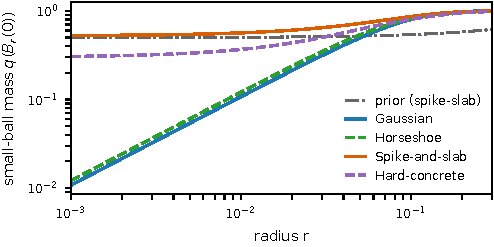
\includegraphics[width=\columnwidth,height=0.20\textheight,keepaspectratio]{results/figures/fig_nn_small_ball.pdf}
    \vspace{-0.4em}
    \caption{\color{blue} Small-ball mass of Bayesian-NN variational posteriors
    (LeNet-5/MNIST): continuous families give $\MI_{\mathrm{pow}}=1$; atom-capable
    families plateau ($\MI_{\mathrm{pow}}=\infty$) at their inclusion atom mass. The
    legend entry ``Horseshoe'' is the mean-field Student-$t$ family above.}
    \label{fig:nn_smallball}
    \vspace{-0.8em}
\end{figure}

% --------------------------- TABLE: Power Mass Index -------------------------
\begin{table}[t!]
\centering
\small
\caption{\color{blue} Power Mass Index of the trained variational posteriors
(LeNet-5/MNIST; network-scale counterpart of Table~\ref{table:MI-common}). Atom mass is
the per-coordinate measure placed at $0$ ($1-\gamma$ for spike-and-slab, $\mathbb
P(z{=}0)$ for hard-concrete).}
\label{tab:nn_mi}
\setlength{\tabcolsep}{4pt}
\renewcommand{\arraystretch}{1.15}
\begin{tabular}{@{}lccc@{}}
\hline
\textbf{Variational family} & atom? & \(\MI_{\mathrm{pow}}\) & atom mass \\
\hline
Gaussian (mean-field) & no  & \(1\)      & \(0\) \\
\add{Student-\(t\)} & no  & \(1\)  & \(0\) \\
Spike-and-slab        & yes & \(\infty\) & \(0.52\) \\
Hard-concrete / \(L_0\) & yes & \(\infty\) & \(0.30\) \\
\hline
\end{tabular}
\end{table}

% --------------------------- FIGURE 2: directional RE-KL ---------------------
\begin{figure}[t!]
    \centering
    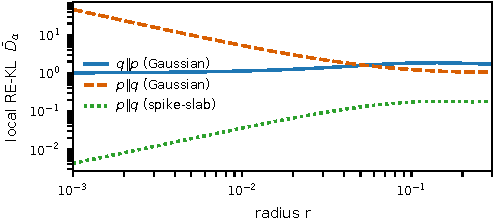
\includegraphics[width=\columnwidth,height=0.19\textheight,keepaspectratio]{results/figures/fig_nn_directional_rekl.pdf}
    \vspace{-0.4em}
    \caption{\color{blue} Directional local RE-KL between variational posteriors and the
    prior: the $\pi_0\|q$ direction diverges for a continuous $q$ (atom not matched) but
    stays bounded for the spike-and-slab $q$ (atom matched), illustrating
    Theorem~\ref{thm:one-sided-MI-pow}.}
    \label{fig:nn_directional}
    \vspace{-0.8em}
\end{figure}
